\section{Results and Discussion} \label{s:results}
This section will present the results of the work and discuss their significance. The piston valve is first compared to the previous results using the rupture disks to ensure the valve works as intended and provides the desired pressurization. The two piston valve iterations are compared to each other to see improvements; and the piston valve is compared to itself to determine reliability and consistency.

% subsection about piston v rupture disk
\subsection{Piston Valve Compared to Rupture Disk} \label{s:disk v piston}
The rupture disks were used in the HENRI system to determine if the system was capable of pressurizing to \SI{1724}{\kilo\pascal} (\SI{250}{psi}) in the desired time frame of \SI{5}{\milli\second}\cite{HeNURETH}. One of the goals of the piston valve is to open quickly enough to maintain as close to rupture disk physics as possible. 
%Computational fluid dynamics (CFD) simulations were validated using these experiments \cite{CFDNureth,HENRIATH}[MIGHT NEED DIFF REF HERE].
\Cref{fig:disk v piston} compares the results of a rupture disk test and a piston valve test, both with initial driver tank pressure of [PRESSURE] and intermediate tube diameter of \SI{2.54}{\centi\meter} (\SI{1}{inch}). [MORE discussion of the plot]

% plot goes here -- disk v piston
\begin{figure}[htbp]
    \vspace{16pt}
    \centering
    %\includegraphics{}
    \caption{Comparison of rupture disk and piston valve HENRI tests at an initial pressure of [PRESSURE] and with intermediate tube diameter of \SI{2.54}{\centi\meter} (\SI{1}{inch}).}
    \label{fig:disk v piston}
    \vspace{16pt}
\end{figure}

The pressure evolution in the piston valve test follows what is expected from the rupture disk tests, which demonstrates the piston valve opens fast enough to meet the demands of the HENRI system. [MORE stuff specific to the plot] While a valve will not be as fast as a rupture disk due to needing a signal and having to actuate, this piston valve is fast enough and trades the small loss of speed for re-usability and predictability, which are strong improvements over the rupture disk. As described in \Cref{ss:need for valve}, changing a rupture disk in between every test is not practical or feasible for the HENRI system in TREAT.


% first piston valve design
% the metal to metal seal did not last long -- durability issues, wear on the sealing surface, even with fancy materials; there was a small leak from the driver tank to the test section before the valve was fully open;

% subsection comparing metal-to-metal seal and o-ring plugs
\subsection{Metal-to-Metal Plug Compared to O-ring Plug}
The metal-to-metal plug design did not seal as well as the o-ring design, which led to a leak from the driver tank into the test section before the piston valve opened all the way. The o-ring plug does not have this issue, even at low operating pressures (below \SI{1.72}{\mega\pascal} (\SI{250}{psi})). \Cref{fig:metal vs oring} shows a test using each plug type. The pressure at [INSERT CORRECT POSITION HERE (probably TS1)] for the metal-to-metal seal increases slightly before the other positions, and before the driver tank pressure decreases significantly, showing that with only the pressure of the driver tank holding it closed, the metal-to-metal seal does not work well. In contrast, the o-ring plug is able to maintain the pressure boundary until the valve opens fully, which provides a quick, crisp helium injection.

\begin{figure}
    \vspace{16pt}
    \centering
    %\includegraphics{}
    \caption{Results of tests with an initial pressure of [PRESSURE] for the metal-to-metal plug and the o-ring plug.}
    \label{fig:metal vs oring}
    \vspace{16pt}
\end{figure}

% subsection about predictability
\subsection{Piston Valve Predictability}
The piston valve's operation at a wide range of pressure must be characterized and predictable for the HENRI system's use in TREAT. The valve should be able to maintain its seal at low pressures, around \SI{1724}{\kilo\pascal} (\SI{250}{psi}), and the gas pressurization in the HENRI system must be determinable for any desired operating pressure. \Cref{fig:piston multi} shows the pressure evolution for four HENRI initial pressures: \SI{1724}{\kilo\pascal} (\SI{250}{psi}), \SI{3448}{\kilo\pascal} (\SI{500}{psi}), \SI{5172}{\kilo\pascal} (\SI{750}{psi}), and \SI{6896}{\kilo\pascal} (\SI{1000}{psi}). These plots show the piston valve can seal at a variety of pressures and that the gas physics are maintained over this pressure range.

\begin{figure}[htbp]
    \vspace{16pt}
    \centering
    \begin{subfigure}{0.49\textwidth}
        \centering
        \includegraphics[width=\textwidth]{results/plots/270psi_MPa_25.png}
        \caption{\SI{1724}{\kilo\pascal} (\SI{250}{psi})}
        \label{fig:piston multi 250}
    \end{subfigure}
    \hfill
    \begin{subfigure}{0.49\textwidth}
        \centering
        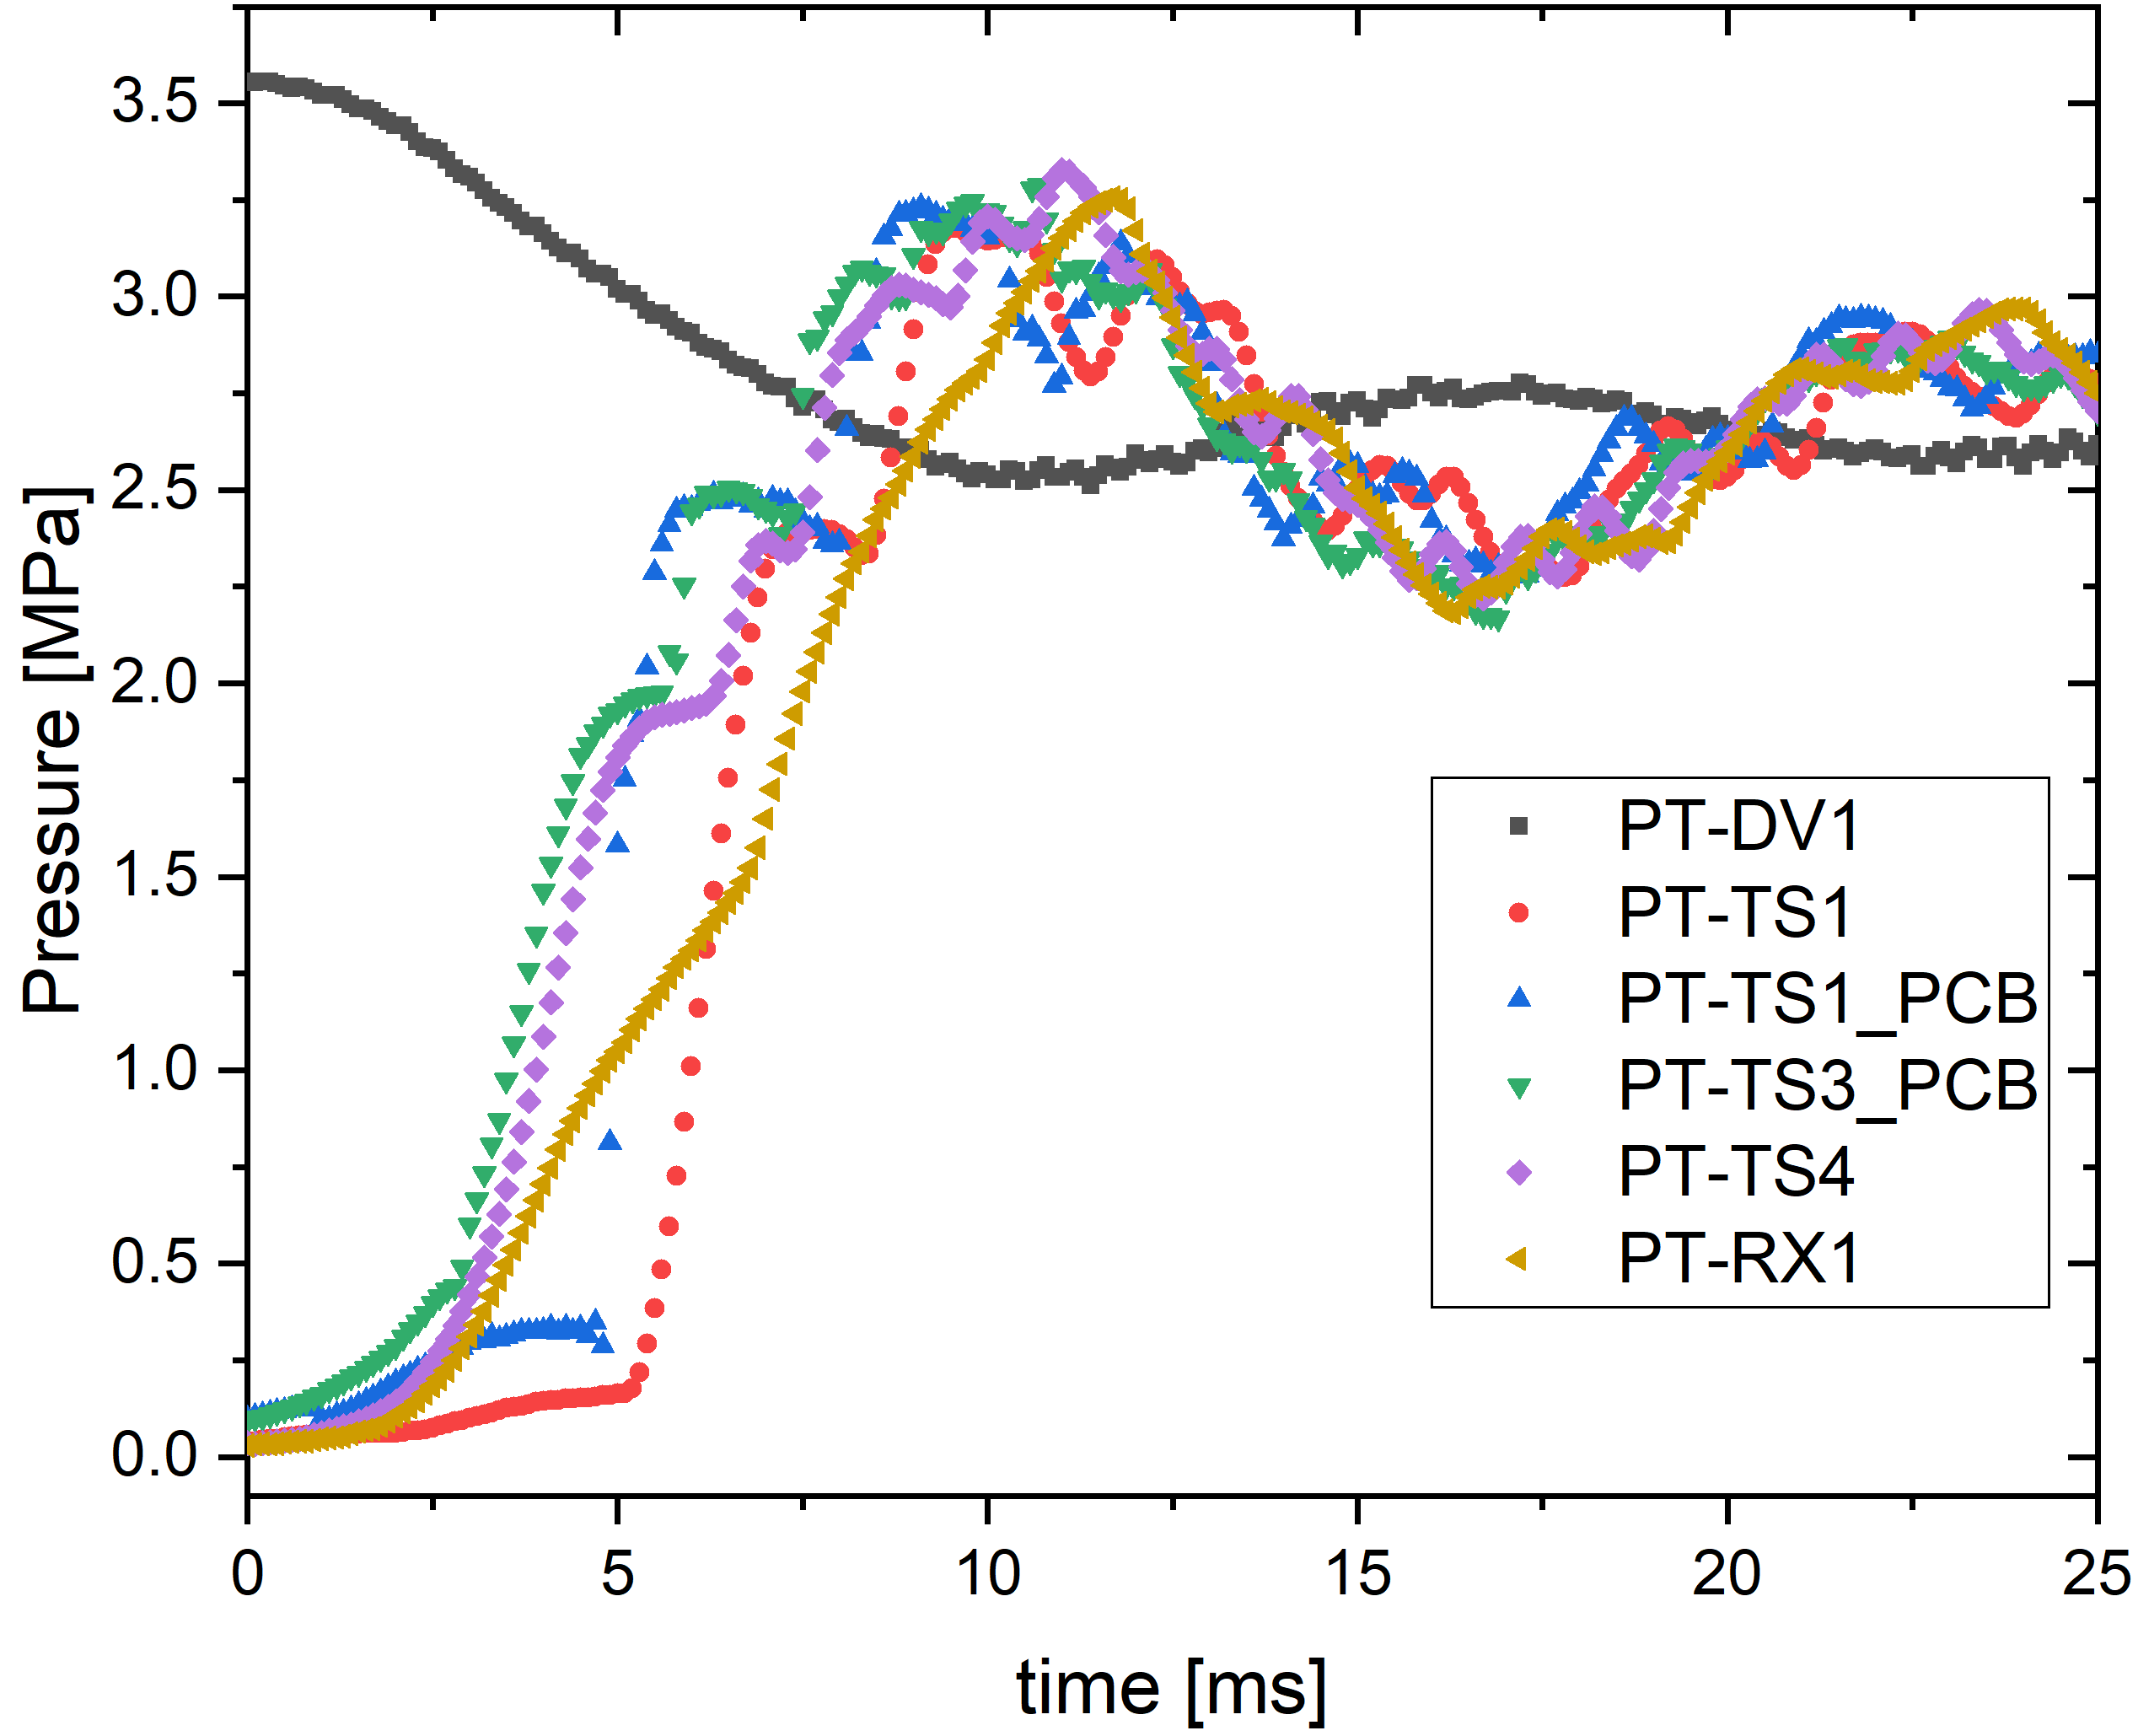
\includegraphics[width=\textwidth]{results/plots/500psi_Mpa_25.png}
        \caption{\SI{3448}{\kilo\pascal} (\SI{500}{psi})}
        \label{fig:piston multi 500}
    \end{subfigure}
    
    \vspace{8pt}
    \begin{subfigure}{0.49\textwidth}
        \centering
        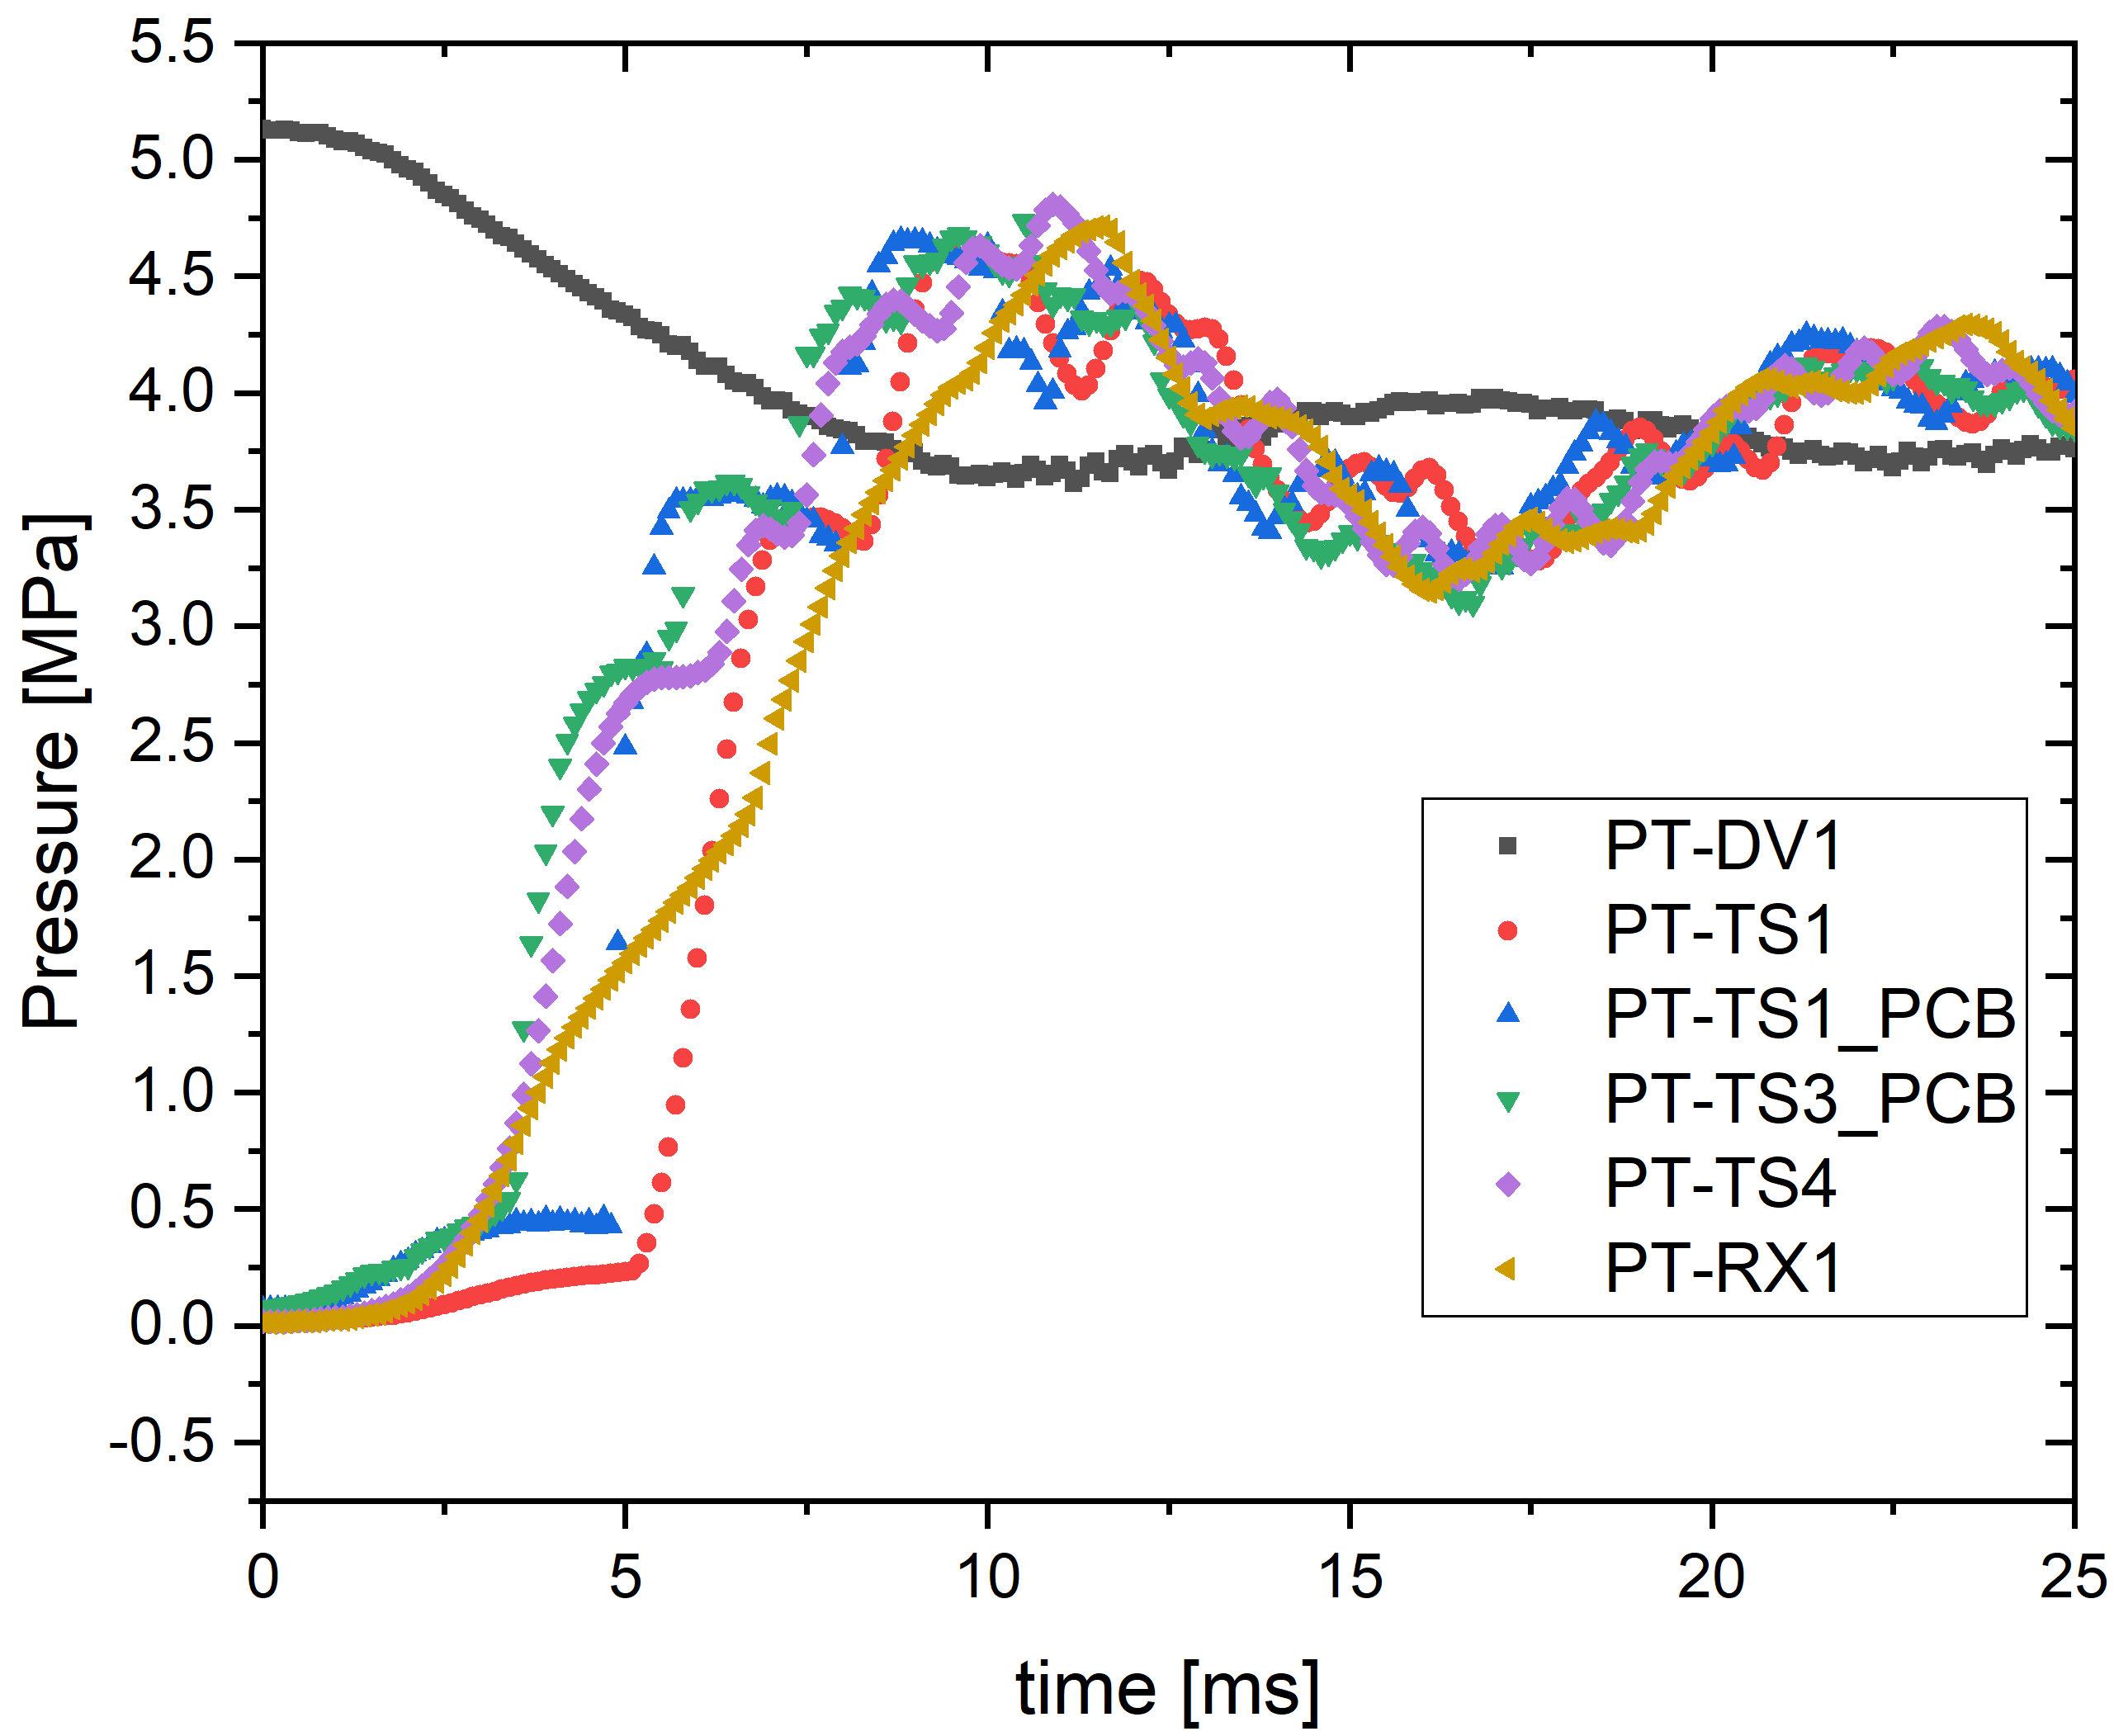
\includegraphics[width=\textwidth]{results/plots/750psi_Mpa_25.png}
        \caption{\SI{5172}{\kilo\pascal} (\SI{750}{psi})}
        \label{fig:piston multi 750}
    \end{subfigure}
    \hfill
    \begin{subfigure}{0.49\textwidth}
        \centering
        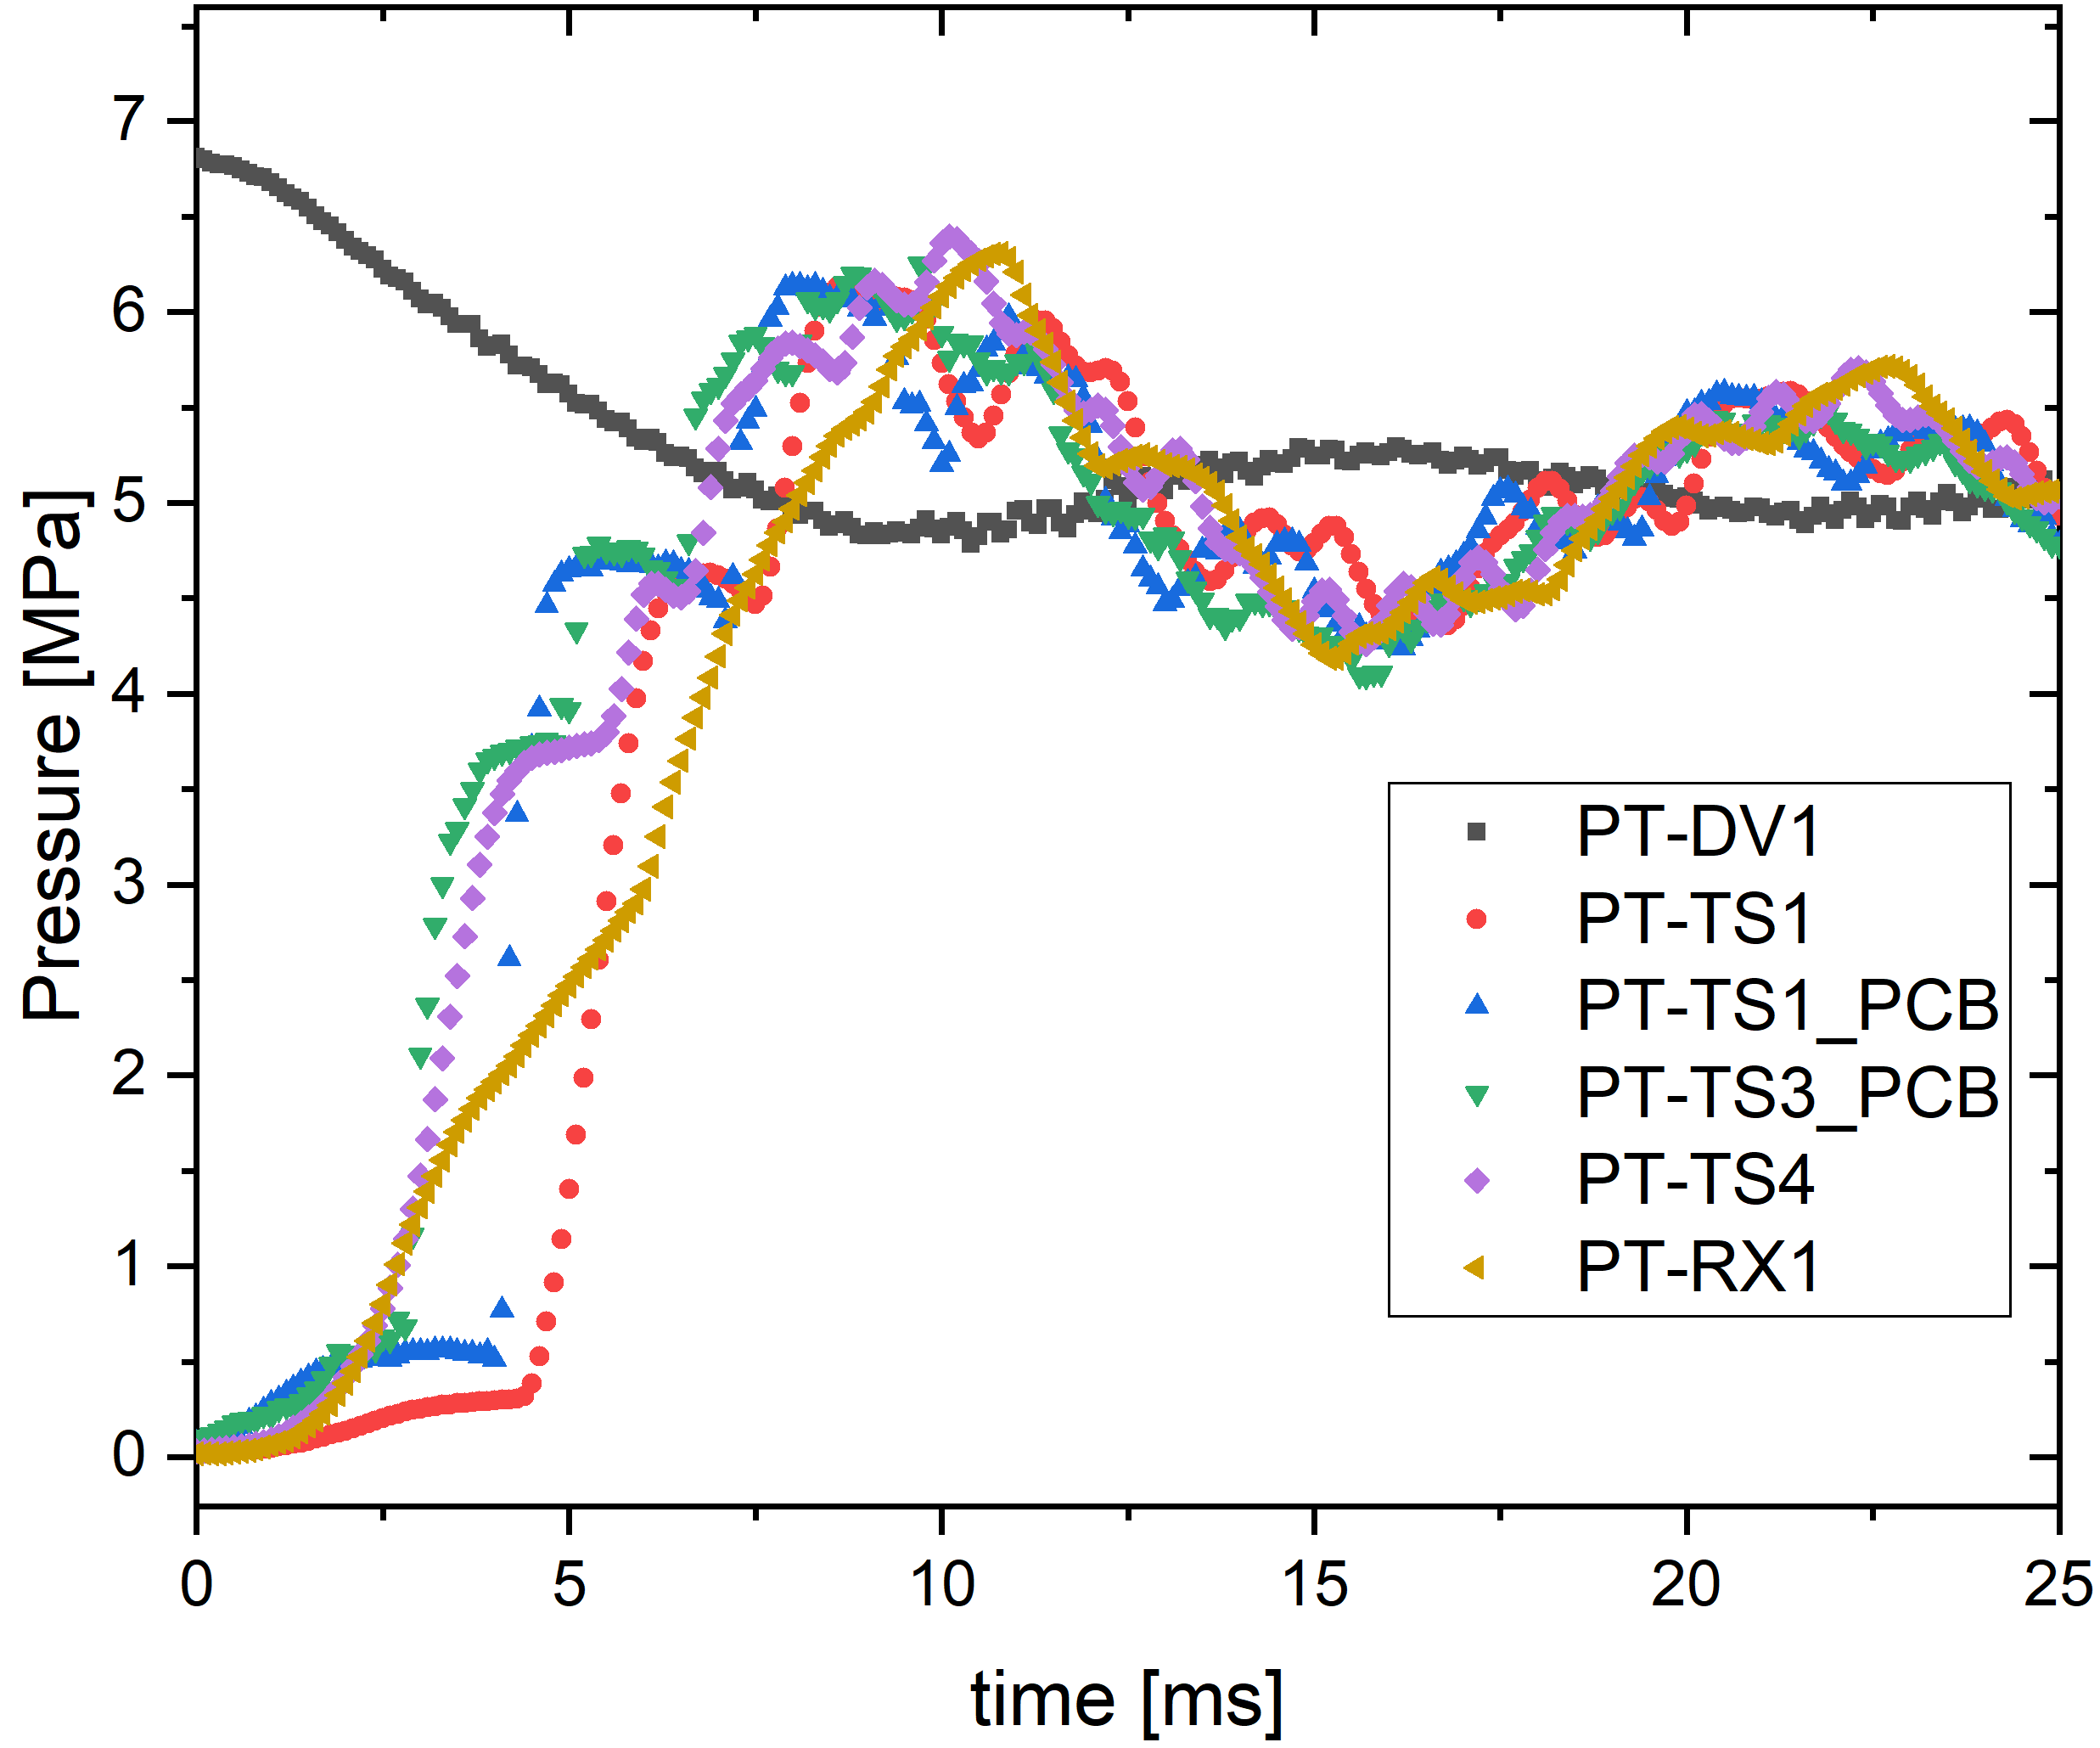
\includegraphics[width=\textwidth]{results/plots/1000psi_Mpa_25.png}
        \caption{\SI{6896}{\kilo\pascal} (\SI{1000}{psi})}
        \label{fig:piston multi 1000}
    \end{subfigure}

    \caption{Pressure evolution for HENRI tests beginning at pressures ranging from \SI{1724}{\kilo\pascal} (\SI{250}{psi}) to \SI{6896}{\kilo\pascal} (\SI{1000}{psi}).}
    \label{fig:piston multi}
    \vspace{16pt}
\end{figure}

Being able to predict the response of the piston valve and the HENRI system as a whole for varying initial pressures is vital for the operation of TREAT. \Cref{fig:piston multi} shows how the system works over a range of pressures, however, it is equally important that the system performs the same for every run at one pressure. \Cref{fig:piston rel} shows the pressure evolution for a range of sensors along the length of the HENRI test section for two[OR MORE] different tests using the piston valve.


\begin{figure}[htbp]
    \vspace{16pt}
    \centering
    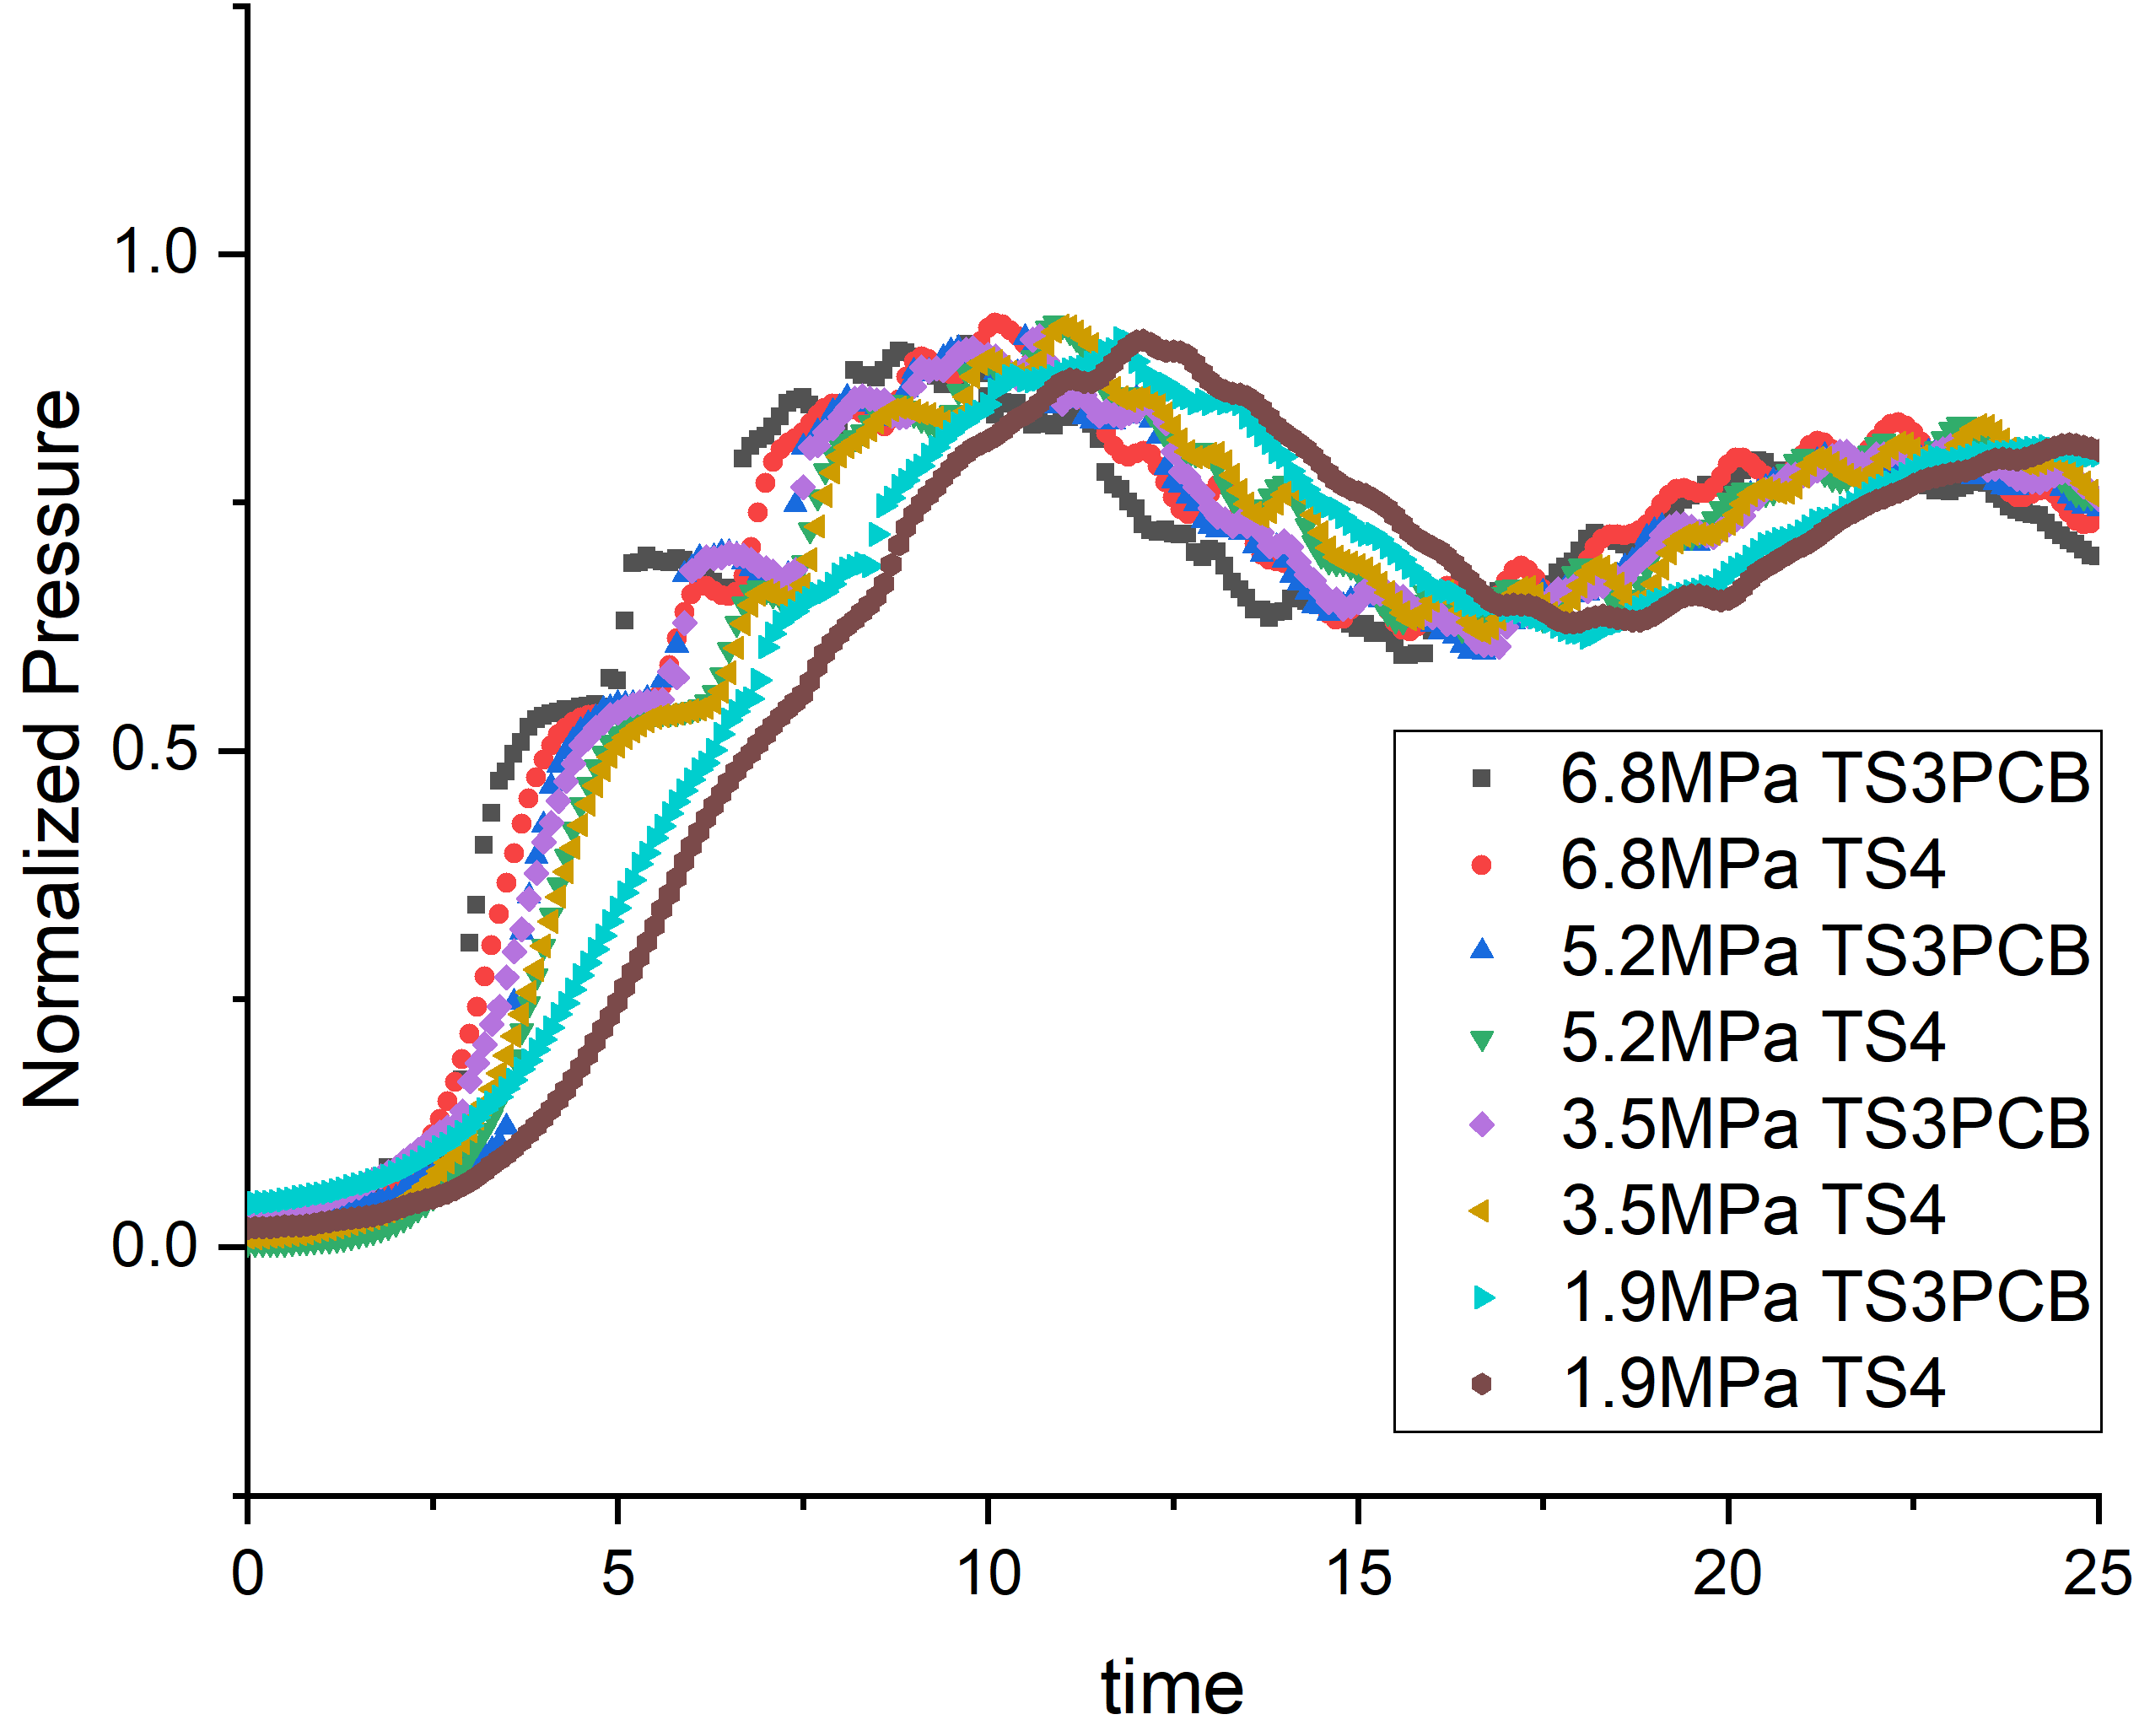
\includegraphics[width=\textwidth]{results/plots/normalized_FFKM.png}
    \caption{Pressure evolution for four normalized tests at a selection of senors along the HENRI test section.}
    \label{fig:piston rel}
    \vspace{16pt}
\end{figure}

The two tests overlap each other quite well, and in some places, it can be difficult to see that two tests are recorded. Dividing the recorded pressure data by the starting driver pressure normalizes the plots, and the curves still overlap regardless of a deviation in pressure. The close overlap of the data for different tests with the piston valve demonstrate the valve's consistency, which will be invaluable for HENRI operation in TREAT.


\begin{figure}[htbp]
    \vspace{16pt}
    \centering
    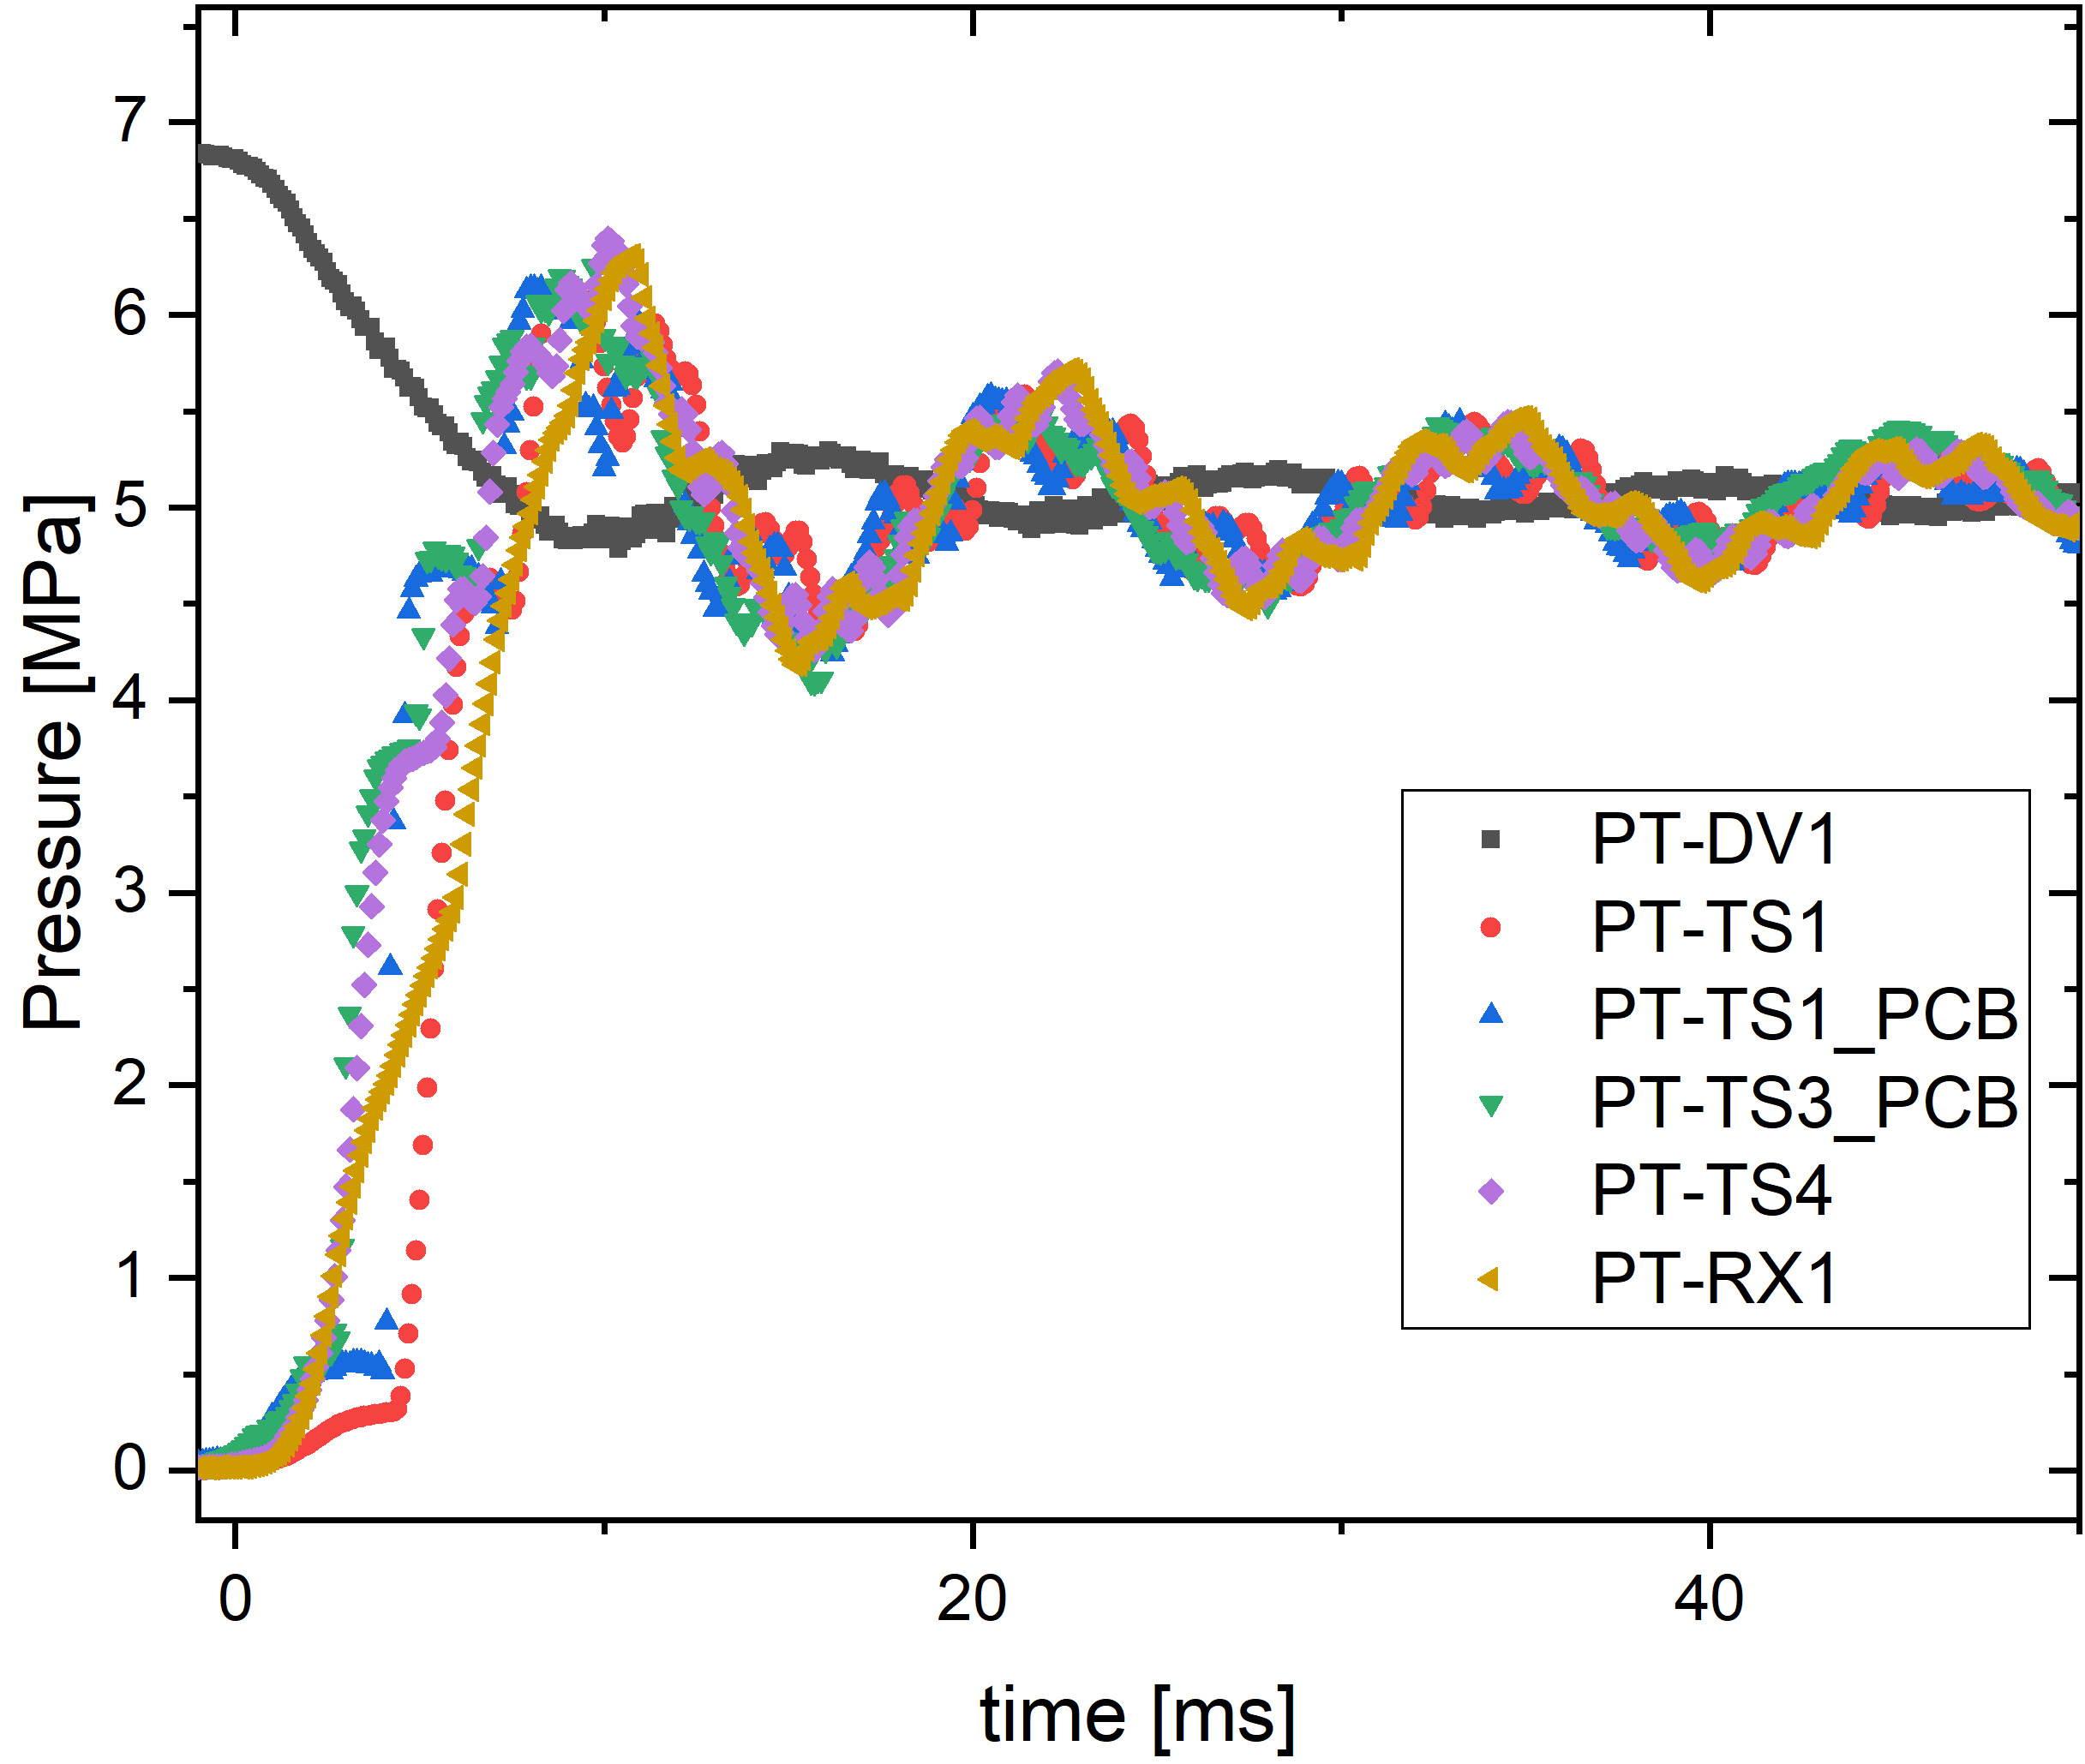
\includegraphics[width=\textwidth]{results/plots/1000psi_Mpa_50.png}
    \caption{Pressure over time for a test starting at approximately \SI{6896}{\kilo\pascal} (\SI{1000}{psia}) using a FFKM o-ring on the second generation plug design.}
    \label{fig:piston 1000psi 50ms}
    \vspace{16pt}
\end{figure}


